\documentclass[11pt]{article}
\usepackage[margin=1in]{geometry}
\usepackage{amsmath,amssymb,booktabs,graphicx}
\usepackage[section]{placeins}
\usepackage{xeCJK}
\setCJKmainfont{Songti SC}
\setCJKsansfont{PingFang SC}
\usepackage[round]{natbib}
\usepackage[hidelinks]{hyperref}
\usepackage[most]{tcolorbox}
\newtcolorbox{zhbox}{breakable,colback=black!4,colframe=black!4,boxrule=0pt,left=6pt,right=6pt,top=3pt,bottom=3pt,arc=0pt,before skip=2pt,after skip=10pt,fontupper=\linespread{1.2}\selectfont}
\newcommand{\zhfont}{}
\graphicspath{{figures/}}
\setlength{\parindent}{0pt}
\setlength{\parskip}{0.4em}
\setlength{\emergencystretch}{2em}
\raggedbottom
\newcommand{\Rhat}{\hat R}
\title{An information scale for the mixing of the Default BART sampler\\[0.3em]\large 中英对照版（灰底为中文）}
\author{}
\date{5 November 2026}
\begin{document}
\maketitle
\vspace{-1.5em}
\section{Question\quad{\zhfont 问题}}
In the paper's two-budget comparison (Section~3), Default chains still disagree after $10^7$ iterations on some settings and agree on others. Sample size alone does not order the settings: Airfoil ($N=1503$) remains elevated, whereas Abalone ($N=4177$) resolves. \citet{tan2024computational} attribute slow convergence of BART samplers to large $n$ and high signal-to-noise ratio. This note asks whether the two factors act through a single quantity, and whether that quantity orders the settings used in the paper. Section~\ref{sec:long-pt} reports the long MTMH+PT chains on SeoulBike.

\begin{zhbox}
论文第 3 节比较了两种预算。跑到 $10^7$ 次迭代后，Default 链在一些 setting 上仍然不一致，在另一些上已经一致。只看样本量排不出这个顺序：Airfoil（$N=1503$）仍然偏高，Abalone（$N=4177$）却已经收敛。Tan et al.\ (2024) 把 BART 采样器收敛慢归因于大 $n$ 和高信噪比。本文要回答两个问题：这两个因素是不是通过同一个量起作用；这个量能不能把论文里的各个 setting 排出顺序。第 \ref{sec:long-pt} 节报告 SeoulBike 上的长 MTMH+PT 链。
\end{zhbox}


\section{A likelihood scale for structural moves\quad{\zhfont 结构移动的似然尺度}}
\label{sec:scale}
Consider an update of tree $j$ with partial residual $r\in\mathbb R^n$, leaves $\ell$ with $n_\ell$ rows and residual sums $S_\ell$, leaf prior $N(0,\tau^2)$ and noise variance $\sigma^2$. Integrating the leaves gives
\begin{equation}
\log p(r\mid\mathcal T_j,\sigma^2) = -\frac{n}{2}\log(2\pi\sigma^2) - \frac{1}{2\sigma^2}\Bigl[\sum_i r_i^2 - \sum_\ell \frac{S_\ell^2}{n_\ell+\sigma^2/\tau^2}\Bigr] - \frac12\sum_\ell \log\Bigl(1+\frac{n_\ell\tau^2}{\sigma^2}\Bigr).
\label{eq:collapsed}
\end{equation}
When $n_\ell\gg\sigma^2/\tau^2$, the bracket is the residual sum of squares $\mathrm{RSS}(\mathcal T_j)$ after fitting leaf means. A structural proposal then changes the log likelihood by
\begin{equation}
\Delta\log p \approx -\frac{\Delta\mathrm{RSS}}{2\sigma^2} + O\Bigl(\log\frac{n_\ell\tau^2}{\sigma^2}\Bigr)\ \text{per leaf added or removed}.
\end{equation}
Write $\Delta\mathrm{RSS}=n s_y^2\,\delta$, where $s_y^2$ is the training variance of $y$ and $\delta$ is the change in the in-sample unexplained fraction. Near stationarity $\sigma^2\approx(1-R^2)s_y^2$, so
\begin{equation}
\Delta\log p \approx -\frac{\kappa}{2}\,\delta,\qquad \kappa=\frac{n}{1-R^2}=n\,(1+\mathrm{SNR}),
\label{eq:kappa}
\end{equation}
with $\mathrm{SNR}=R^2/(1-R^2)$. The tree prior ratio and the proposal ratio do not depend on $n$ or $\sigma^2$, and the leaf term grows only logarithmically. A move that worsens the fit by $\delta>0$ is therefore accepted with probability at most of order $\exp(-\kappa\delta/2)$, up to factors that do not depend on $\kappa$.

A change in the decomposition of the ensemble generally passes through intermediate states with a worse fit. If the required loss $\delta^\ast$ is similar across datasets, the crossing rate decreases like $\exp(-\kappa\delta^\ast/2)$, and $\kappa$ sets the difficulty. For $\delta^\ast=10^{-4}$, the cost is $0.28$ nats on Abalone ($\kappa\approx5.6\times10^3$), $3.1$ nats on SeoulBike ($\kappa\approx6.3\times10^4$) and $18$ nats on CPU activity ($\kappa\approx3.6\times10^5$). Tempering at temperature $T$ replaces $\kappa$ by $\kappa/T$.

The argument makes two testable predictions:
\begin{enumerate}
\item $\kappa$ orders mixing difficulty across datasets better than $n$ or $1-R^2$ separately.
\item In a regression of a mixing diagnostic on $\log n$ and $\log\{1/(1-R^2)\}$, the two coefficients are equal.
\end{enumerate}

\begin{zhbox}
考虑更新第 $j$ 棵树。记号如下：
\begin{itemize}
\item 偏残差为 $r\in\mathbb R^n$；
\item 叶子 $\ell$ 含 $n_\ell$ 行，残差和为 $S_\ell$；
\item 叶子先验为 $N(0,\tau^2)$，噪声方差为 $\sigma^2$。
\end{itemize}
把叶子值积分掉，得到
\begin{equation*}
\log p(r\mid\mathcal T_j,\sigma^2) = -\frac{n}{2}\log(2\pi\sigma^2) - \frac{1}{2\sigma^2}\Bigl[\sum_i r_i^2 - \sum_\ell \frac{S_\ell^2}{n_\ell+\sigma^2/\tau^2}\Bigr] - \frac12\sum_\ell \log\Bigl(1+\frac{n_\ell\tau^2}{\sigma^2}\Bigr).
\end{equation*}
当 $n_\ell\gg\sigma^2/\tau^2$ 时，方括号就是用叶子均值拟合后的残差平方和 $\mathrm{RSS}(\mathcal T_j)$。于是一个结构提议带来的对数似然变化为
\begin{equation*}
\Delta\log p \approx -\frac{\Delta\mathrm{RSS}}{2\sigma^2} + O\Bigl(\log\frac{n_\ell\tau^2}{\sigma^2}\Bigr)\quad\text{（每增减一个叶子）}.
\end{equation*}
记 $\Delta\mathrm{RSS}=n s_y^2\,\delta$，其中 $s_y^2$ 是训练集 $y$ 的方差，$\delta$ 是样本内"未解释比例"的变化量。接近平稳时 $\sigma^2\approx(1-R^2)s_y^2$，所以
\begin{equation*}
\Delta\log p \approx -\frac{\kappa}{2}\,\delta,\qquad \kappa=\frac{n}{1-R^2}=n\,(1+\mathrm{SNR}),
\end{equation*}
其中 $\mathrm{SNR}=R^2/(1-R^2)$。树先验之比和提议分布之比都与 $n$、$\sigma^2$ 无关，叶子项只按对数增长。因此，一个让拟合变差 $\delta>0$ 的移动，被接受的概率至多是 $\exp(-\kappa\delta/2)$ 的量级，其余因子不随 $\kappa$ 变化。

要改变整个森林的分解方式，一般得经过一些拟合更差的中间状态。如果不同数据集需要付出的损失 $\delta^\ast$ 差不多，跨越的速率就按 $\exp(-\kappa\delta^\ast/2)$ 下降，难度由 $\kappa$ 决定。以 $\delta^\ast=10^{-4}$ 为例，代价分别是：
\begin{itemize}
\item Abalone（$\kappa\approx5.6\times10^3$）：0.28 nat；
\item SeoulBike（$\kappa\approx6.3\times10^4$）：3.1 nat；
\item CPU activity（$\kappa\approx3.6\times10^5$）：18 nat。
\end{itemize}
在温度 $T$ 下升温，相当于把 $\kappa$ 换成 $\kappa/T$。

由此得到两个可检验的预测：
\begin{enumerate}
\item 在不同数据集之间，$\kappa$ 对混合难度的排序比单独的 $n$ 或 $1-R^2$ 更好。
\item 把混合诊断量对 $\log n$ 和 $\log\{1/(1-R^2)\}$ 做回归，两个系数相等。
\end{enumerate}
\end{zhbox}


\section{Settings and measurements\quad{\zhfont 设置与度量}}


\textbf{Settings (48).}
\begin{itemize}
\item The twelve paper settings, with five runs each. The three DART settings use the Default sampler with the Dirichlet splitting prior, as in the paper.
\item The 20 size and noise sweep settings of Section~3, with five runs each.
\item 16 controlled settings on SeoulBike, Airfoil and Abalone, with three runs each, using the store train splits 0--2 and fixed test panels. These keep $X$ and $n$ fixed and replace the response by one of three choices:
\begin{itemize}
\item the observed $y$;
\item $y$ plus independent Gaussian noise;
\item a semi-synthetic response $\hat f(X)+\varepsilon$, with $\varepsilon$ Gaussian and homoskedastic. Here $\hat f$ is a histogram gradient boosting fit (500 iterations) to the full dataset, used as a known regression function.
\end{itemize}
Noise variances are set to reach the target noise fractions in Table~\ref{tab:controlled}.
\end{itemize}

\begin{zhbox}
\textbf{Setting（共 48 个）。}
\begin{itemize}
\item 论文的 12 个 setting，各 5 个 run。三个 DART setting 和论文一样，用带 Dirichlet 分裂先验的 Default 采样器。
\item 论文第 3 节的 20 个规模和噪声扫描 setting，各 5 个 run。
\item 在 SeoulBike、Airfoil 和 Abalone 上的 16 个控制实验，各 3 个 run，用 store 里的训练划分 0--2 和固定测试面板。$X$ 和 $n$ 保持不变，只把响应换成以下三种之一：
\begin{itemize}
\item 观测到的 $y$；
\item $y$ 加独立高斯噪声；
\item 半合成响应 $\hat f(X)+\varepsilon$，$\varepsilon$ 为同方差高斯噪声。其中 $\hat f$ 是用全数据拟合的直方图梯度提升（500 次迭代），作为已知的回归函数。
\end{itemize}
噪声方差按表 \ref{tab:controlled} 里的目标噪声比例设定。
\end{itemize}
\end{zhbox}


\textbf{Mixing diagnostic.} The rank-normalized split $\Rhat$ (ArviZ, as in the paper) is computed at each of the 100 fixed test inputs from four Default chains. As in the paper, every record keeps 7,000 post-warm-up draws per chain:
\begin{itemize}
\item $10^4$-iteration chains: iterations 3,001--10,000;
\item $10^7$-iteration chains: the last 70\% of the stride-1,000 record.
\end{itemize}
The note reports the median over inputs, averaged over runs.

\begin{zhbox}
\textbf{混合诊断。}在 100 个固定测试点上，分别用 4 条 Default 链计算 rank-normalized split $\Rhat$（ArviZ，与论文相同）。和论文一样，每种记录每条链都保留 7,000 个 post-warm-up draws：
\begin{itemize}
\item $10^4$ 次迭代的链：第 3,001--10,000 次迭代；
\item $10^7$ 次迭代的链：stride 1,000 记录的后 70\%。
\end{itemize}
报告的是各测试点的中位数，再对 run 取平均。
\end{zhbox}


\textbf{Noise fraction.} $1-R^2_{\mathrm{CV}}$ is the 5-fold cross-validated mean squared error of histogram gradient boosting on the training set, divided by $s_y^2$. It requires no MCMC. The posterior alternative is $\bar\sigma^2/s_y^2$, computed from the same retained Default draws; correlations with both are reported.

\begin{zhbox}
\textbf{噪声比例。}$1-R^2_{\mathrm{CV}}$ 是在训练集上做 5 折交叉验证的梯度提升均方误差，除以 $s_y^2$，不需要跑 MCMC。另一种取法是后验的 $\bar\sigma^2/s_y^2$，用同样保留的 Default draws 计算。两种都报告了相关系数。
\end{zhbox}


\textbf{Acceptance rates.} One Default chain per setting (run 0) is used. The acceptance rate is the number of accepted proposals divided by the number of valid proposals, over iterations $3{,}001$--$5{,}000$.

\begin{zhbox}
\textbf{接受率。}每个 setting 用一条 Default 链（run 0）。接受率是第 3,001--5,000 次迭代中，被接受的提议数除以有效提议数。
\end{zhbox}


\section{Results\quad{\zhfont 结果}}


\subsection{Ordering across settings\quad{\zhfont 跨 setting 的排序}}
Figure~\ref{fig:kappa}(a) plots $\Rhat-1$ against $\kappa$ for all 48 settings, and Table~\ref{tab:spearman} gives the rank correlations. $\kappa$ gives $\rho=0.89$, compared with $0.66$ for $n$ and $0.60$ for $1/(1-R^2_{\mathrm{CV}})$. On the twelve paper settings at $10^7$ iterations, $\rho=0.86$ for $\kappa$ and $0.57$ for $n$.

Table~\ref{tab:paper} lists the paper settings by $\kappa$:
\begin{itemize}
\item Airfoil and Abalone, which have similar $N$ but opposite outcomes, differ threefold in $\kappa$.
\item CalHousing, Friedman and Airfoil have nearly equal $\kappa$ and similar $10^4$-iteration $\Rhat$.
\item The four settings that remain above $1.1$ after $10^7$ iterations have the four largest values of $\kappa$.
\item The three DART settings share $n$ and the noise level with Friedman. Their posterior noise fraction is the same ($0.037$ against $0.036$), and their $\Rhat$ is close to Friedman's (1.17--1.20 against 1.23). Their cross-validated $\kappa$ is lower (1.2--1.6$\times10^4$) because the gradient-boosting error grows with the number of nuisance predictors.
\end{itemize}

\begin{zhbox}
图 \ref{fig:kappa}(a) 画出了全部 48 个 setting 的 $\Rhat-1$ 对 $\kappa$，表 \ref{tab:spearman} 给出秩相关。$\kappa$ 的 $\rho=0.89$，$n$ 只有 0.66，$1/(1-R^2_{\mathrm{CV}})$ 只有 0.60。在 12 个论文 setting 的 $10^7$ 次迭代结果上，$\kappa$ 是 0.86，$n$ 是 0.57。

表 \ref{tab:paper} 把论文 setting 按 $\kappa$ 排列：
\begin{itemize}
\item Airfoil 和 Abalone 的 $N$ 相近、结果相反，两者的 $\kappa$ 相差三倍。
\item CalHousing、Friedman 和 Airfoil 的 $\kappa$ 几乎相同，$10^4$ 次迭代的 $\Rhat$ 也相近。
\item $10^7$ 次迭代后仍高于 1.1 的四个 setting，正好是 $\kappa$ 最大的四个。
\item 三个 DART setting 和 Friedman 的 $n$、噪声水平都相同。它们的后验噪声比例一样（0.037 对 0.036），$\Rhat$ 也接近 Friedman（1.17--1.20 对 1.23）。它们交叉验证得到的 $\kappa$ 偏低（1.2--1.6$\times10^4$），原因是梯度提升的误差会随无关变量增多而变大。
\end{itemize}
\end{zhbox}


\begin{table}[h]
\centering
\caption{Spearman correlation of median pointwise $\Rhat$ with candidate scales.\newline{\zhfont 中位 pointwise $\Rhat$ 与各候选尺度的 Spearman 相关。}}
\label{tab:spearman}
\begin{tabular}{lccc}
\toprule
Scale & 48 settings, $10^4$ its & 48 settings, $10^4$ its & 12 paper settings, $10^7$ its \\
 & ($1-R^2_{\mathrm{CV}}$) & ($\bar\sigma^2/s_y^2$) & ($1-R^2_{\mathrm{CV}}$) \\
\midrule
$\kappa=n/(1-R^2)$ & 0.89 & 0.89 & 0.86 \\
$n$ & 0.66 & 0.66 & 0.57 \\
$1/(1-R^2)$ & 0.60 & 0.44 & 0.42 \\
\bottomrule
\end{tabular}
\end{table}

\begin{table}[h]
\centering
\caption{Paper settings ordered by $\kappa$. $n$ is the training size; $\Rhat$ is the median pointwise value averaged over five runs. The last column gives the acceptance rate of change moves.\newline{\zhfont 按 $\kappa$ 排序的论文 setting。$n$ 为训练集大小；$\Rhat$ 为中位 pointwise 值，对 5 个 run 取平均；最后一列是 change 移动的接受率。}}
\label{tab:paper}
\begin{tabular}{lrrrccc}
\toprule
Setting & $n$ & $1-R^2_{\mathrm{CV}}$ & $\kappa$ & $\Rhat$, $10^4$ & $\Rhat$, $10^7$ & change acc. \\
\midrule
Abalone & 3{,}057 & 0.543 & 5{,}629 & 1.097 & 1.000 & 0.163 \\
Concrete & 697 & 0.083 & 8{,}436 & 1.173 & 1.003 & 0.136 \\
DART $d{=}200$ & 1{,}425 & 0.117 & 12{,}219 & 1.184 & 1.000 & 0.099 \\
DART $d{=}100$ & 1{,}425 & 0.107 & 13{,}327 & 1.173 & 1.000 & 0.088 \\
DART $d{=}20$ & 1{,}425 & 0.091 & 15{,}644 & 1.199 & 1.000 & 0.104 \\
Friedman & 1{,}425 & 0.083 & 17{,}217 & 1.233 & 1.002 & 0.136 \\
Airfoil & 1{,}052 & 0.060 & 17{,}420 & 1.298 & 1.041 & 0.112 \\
CalHousing & 3{,}675 & 0.205 & 17{,}958 & 1.251 & 1.018 & 0.105 \\
Superconduct & 3{,}675 & 0.139 & 26{,}517 & 1.441 & 1.234 & 0.062 \\
SeoulBike & 6{,}495 & 0.103 & 62{,}812 & 1.466 & 1.318 & 0.061 \\
CCPP & 7{,}101 & 0.036 & 194{,}668 & 1.439 & 1.126 & 0.043 \\
CPU activity & 6{,}069 & 0.017 & 364{,}149 & 1.518 & 1.236 & 0.031 \\
\bottomrule
\end{tabular}
\end{table}

\begin{figure}[h]
\centering
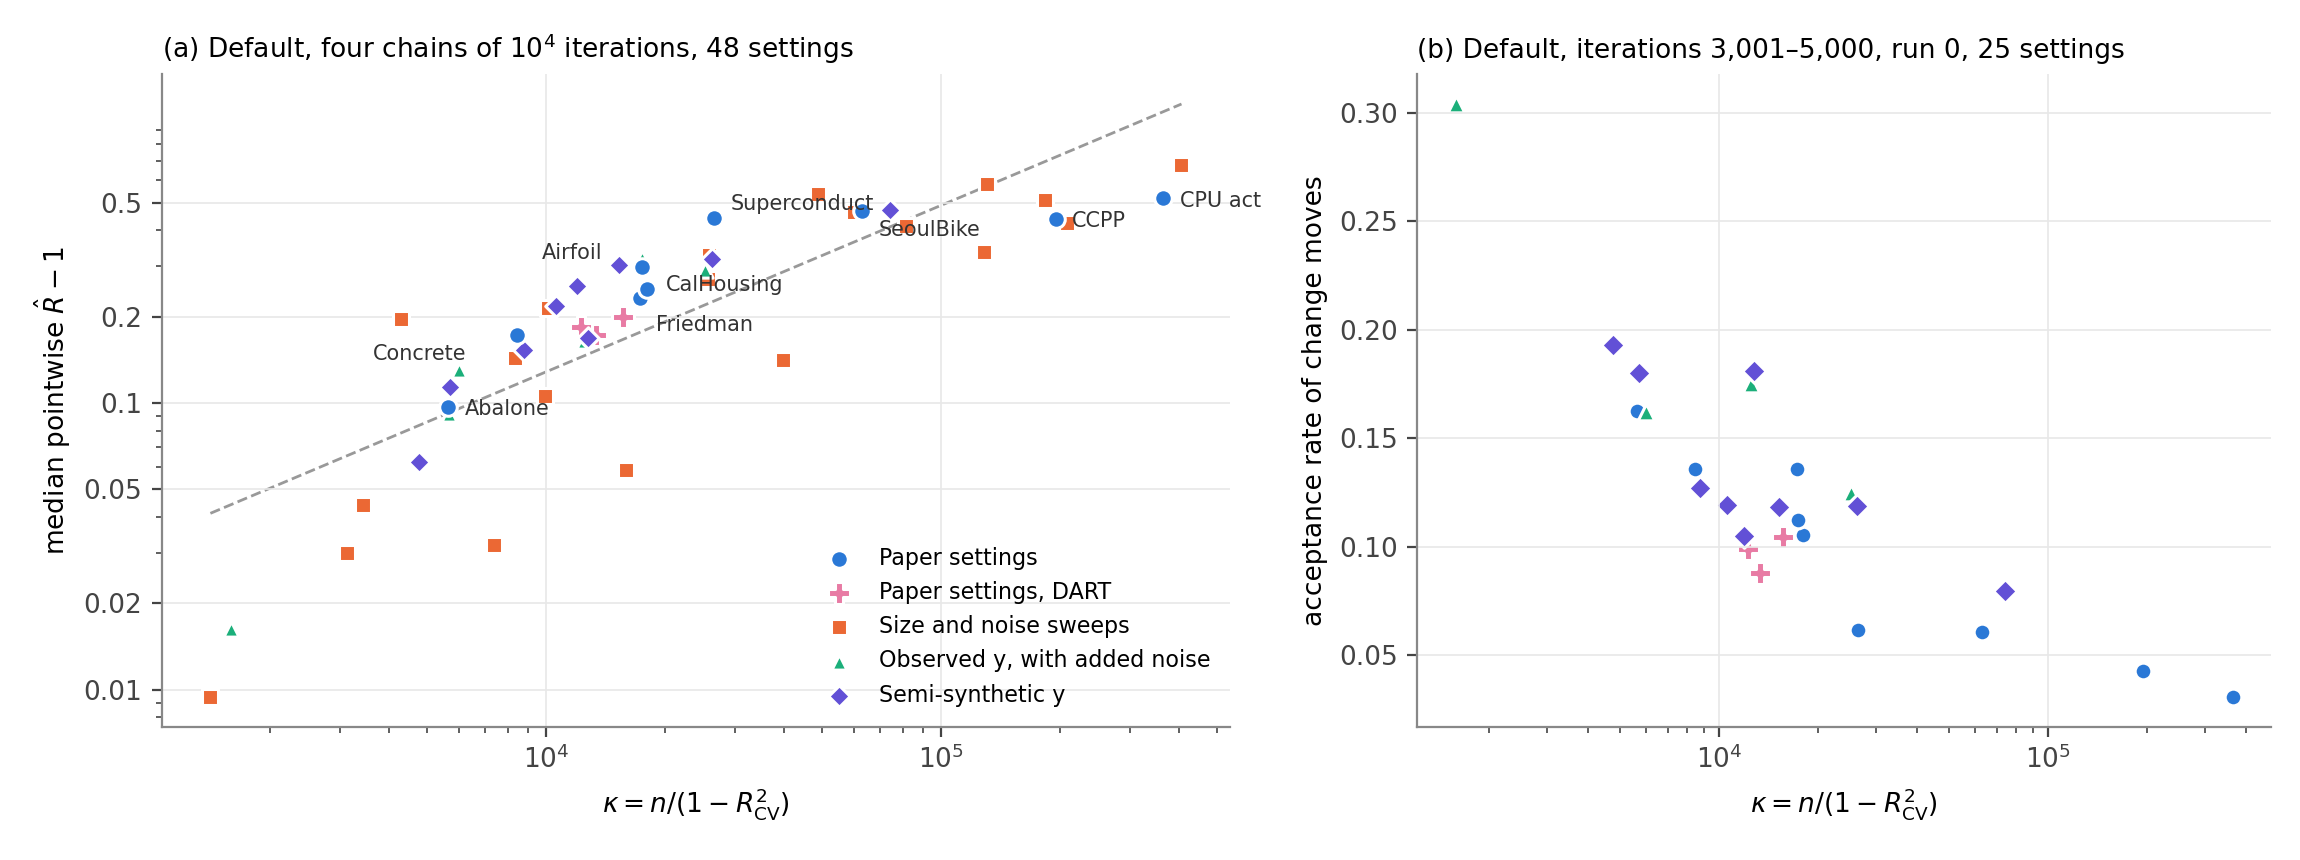
\includegraphics[width=\linewidth]{rhat_vs_kappa.png}
\caption{(a) Median pointwise $\Rhat-1$ against $\kappa$ for 48 settings, on logarithmic axes. The dashed line is the least-squares fit $\log(\Rhat-1)=0.58\log\kappa-7.40$. (b) Acceptance rate of Default change moves against $\kappa$, one chain per setting; markers as in (a).\newline{\zhfont (a) 48 个 setting 的中位 pointwise $\Rhat-1$ 对 $\kappa$，双对数坐标。虚线是最小二乘拟合 $\log(\Rhat-1)=0.58\log\kappa-7.40$。(b) Default 的 change 移动接受率对 $\kappa$，每个 setting 一条链；图例同 (a)。}}
\label{fig:kappa}
\end{figure}

\subsection{Do $n$ and the noise fraction enter only through $\kappa$?\quad{\zhfont $n$ 和噪声比例是否只通过 $\kappa$ 起作用？}}
Over the 48 settings, fit the regression
\[
\log(\Rhat-1)=a\log n+b\log\{1/(1-R^2)\}+c .
\]
With $1-R^2_{\mathrm{CV}}$ it gives $a=0.61\pm0.08$ and $b=0.55\pm0.09$. With $\bar\sigma^2/s_y^2$ it gives $a=0.72\pm0.08$ and $b=0.55\pm0.07$, a gap of about 1.6 combined standard errors. The standard errors are from ordinary least squares.

Constraining $a=b$, that is regressing on $\log\kappa$ alone, barely changes the coefficient of determination: 0.68 versus 0.68 with $1-R^2_{\mathrm{CV}}$, and 0.71 versus 0.73 with $\bar\sigma^2/s_y^2$. By comparison, $\log n$ alone gives 0.40 and $\log\{1/(1-R^2_{\mathrm{CV}})\}$ alone gives 0.32. Within this range, a change in $n$ and a change in the noise fraction have nearly the same effect when they change $\kappa$ by the same factor.

\begin{zhbox}
在 48 个 setting 上拟合回归
\[
\log(\Rhat-1)=a\log n+b\log\{1/(1-R^2)\}+c .
\]
\begin{itemize}
\item 用 $1-R^2_{\mathrm{CV}}$：$a=0.61\pm0.08$，$b=0.55\pm0.09$。
\item 用 $\bar\sigma^2/s_y^2$：$a=0.72\pm0.08$，$b=0.55\pm0.07$，两者相差约 1.6 个合并标准误。
\end{itemize}
标准误来自普通最小二乘。

限制 $a=b$，也就是只对 $\log\kappa$ 回归，决定系数几乎不变：用 $1-R^2_{\mathrm{CV}}$ 时是 0.68 对 0.68，用 $\bar\sigma^2/s_y^2$ 时是 0.71 对 0.73。作为对比，只用 $\log n$ 是 0.40，只用 $\log\{1/(1-R^2_{\mathrm{CV}})\}$ 是 0.32。在这个范围内，只要把 $\kappa$ 改变同样的倍数，改 $n$ 和改噪声比例的效果几乎相同。
\end{zhbox}


\subsection{Observed and semi-synthetic responses\quad{\zhfont 观测响应与半合成响应}}
Table~\ref{tab:controlled} holds $X$ and $n$ fixed. At matched noise fractions, the observed response and the semi-synthetic response give nearly equal $\Rhat$:
\begin{itemize}
\item SeoulBike: 1.484 and 1.472; 1.291 and 1.318; 1.165 and 1.168;
\item Airfoil: 1.321 and 1.303; 1.130 and 1.114.
\end{itemize}
The semi-synthetic response is homoskedastic, Gaussian and has a known regression function. Features of the observed responses, such as count-valued and heteroskedastic SeoulBike rentals, are therefore not needed to produce the observed disagreement. The value of $\kappa$ suffices.

For Abalone, $\hat f$ contains structure that 3,057 rows do not identify. The attainable $1-R^2_{\mathrm{CV}}$ therefore stays near 0.26 at the smallest design noise. Measured by the attainable $\kappa$, these settings follow the same ordering.

\begin{zhbox}
表 \ref{tab:controlled} 固定了 $X$ 和 $n$。在相同的噪声比例下，观测响应和半合成响应给出几乎相同的 $\Rhat$：
\begin{itemize}
\item SeoulBike：1.484 和 1.472；1.291 和 1.318；1.165 和 1.168；
\item Airfoil：1.321 和 1.303；1.130 和 1.114。
\end{itemize}
半合成响应是同方差、高斯的，回归函数已知。所以观测数据的特殊之处，例如 SeoulBike 租车量是计数、异方差，并不是产生链间不一致的必要条件，$\kappa$ 的大小就足够了。

Abalone 的 $\hat f$ 含有一些 3,057 行数据识别不出来的结构，所以即使设定的噪声最小，可达到的 $1-R^2_{\mathrm{CV}}$ 也停在 0.26 左右。按可达到的 $\kappa$ 来衡量，这些 setting 仍然符合同样的排序。
\end{zhbox}


\begin{table}[h]
\centering
\caption{Controlled settings: mean over three runs; acceptance from run 0. ``Target'' is the design noise fraction.\newline{\zhfont 控制实验：3 个 run 的平均；接受率来自 run 0。"目标"是设计的噪声比例。}}
\label{tab:controlled}
\begin{tabular}{llcccrc}
\toprule
Data & Response & Target & $1-R^2_{\mathrm{CV}}$ & $\kappa$ & $\Rhat$, $10^4$ & change acc. \\
\midrule
SeoulBike & observed & -- & 0.102 & 63{,}553 & 1.484 & 0.061 \\
SeoulBike & semi-synthetic & 0.042 & 0.088 & 73{,}993 & 1.472 & 0.079 \\
SeoulBike & observed + noise & 0.17 & 0.258 & 25{,}218 & 1.291 & 0.125 \\
SeoulBike & semi-synthetic & 0.17 & 0.247 & 26{,}320 & 1.318 & 0.119 \\
SeoulBike & observed + noise & 0.4 & 0.520 & 12{,}484 & 1.165 & 0.175 \\
SeoulBike & semi-synthetic & 0.4 & 0.509 & 12{,}755 & 1.168 & 0.181 \\
\midrule
Airfoil & observed & -- & 0.060 & 17{,}434 & 1.321 & 0.112 \\
Airfoil & semi-synthetic & 0.025 & 0.069 & 15{,}242 & 1.303 & 0.118 \\
Airfoil & observed + noise & 0.1 & 0.175 & 6{,}004 & 1.130 & 0.162 \\
Airfoil & semi-synthetic & 0.1 & 0.184 & 5{,}709 & 1.114 & 0.180 \\
Airfoil & observed + noise & 0.4 & 0.663 & 1{,}586 & 1.016 & 0.304 \\
\midrule
Abalone & observed & -- & 0.540 & 5{,}666 & 1.092 & 0.163 \\
Abalone & semi-synthetic & 0.38 & 0.642 & 4{,}760 & 1.062 & 0.193 \\
Abalone & semi-synthetic & 0.1 & 0.348 & 8{,}784 & 1.153 & 0.127 \\
Abalone & semi-synthetic & 0.04 & 0.288 & 10{,}600 & 1.217 & 0.119 \\
Abalone & semi-synthetic & 0.01 & 0.256 & 11{,}958 & 1.255 & 0.105 \\
\bottomrule
\end{tabular}
\end{table}

\subsection{Acceptance rates\quad{\zhfont 接受率}}
Equation~\eqref{eq:kappa} implies that, at stationarity, a larger share of proposals is rejected as $\kappa$ grows. Over the 25 paper and controlled settings with measured rates, Spearman correlations with $\kappa$ are $-0.80$ (grow), $-0.75$ (prune), $-0.79$ (change) and $-0.73$ (swap). Change-move acceptance falls from 0.30 at $\kappa\approx1.6\times10^3$ to 0.03 at $\kappa\approx3.6\times10^5$ (Figure~\ref{fig:kappa}(b)). At fixed $X$, adding noise raises every rate; on SeoulBike, change acceptance rises from 0.061 to 0.175.

\begin{zhbox}
式 \eqref{eq:kappa} 意味着，在平稳状态下，$\kappa$ 越大，被拒绝的提议比例越高。在测了接受率的 25 个论文和控制 setting 上，四种移动的接受率与 $\kappa$ 的 Spearman 相关分别是：grow $-0.80$，prune $-0.75$，change $-0.79$，swap $-0.73$。change 移动的接受率从 $\kappa\approx1.6\times10^3$ 时的 0.30，降到 $\kappa\approx3.6\times10^5$ 时的 0.03（图 \ref{fig:kappa}(b)）。在 $X$ 固定时，加噪声会提高所有接受率；SeoulBike 上，change 的接受率从 0.061 升到 0.175。
\end{zhbox}


\section{Long MTMH+PT chains on SeoulBike\quad{\zhfont SeoulBike 上的长 MTMH+PT 链}}
\label{sec:long-pt}


\textbf{Setup.}
\begin{itemize}
\item Data: SeoulBike, run 0, with the same training split and fixed test panel as the short chains.
\item Chains: four independent MTMH+PT chains ($K=10$) of $10^6$ iterations each.
\item Tempering: the 46-temperature run-0 ladder of the short-chain search ($T$ from 1 to 100), exchanges every 50 iterations, one worker per temperature.
\item Execution: each chain runs in 100 chunks of $10^4$ iterations, and each chunk continues from the final states of the previous one. Seeds follow the long-chain convention $2024+100{,}000+\text{chain}$; the code is commit \texttt{e86f19d}.
\item Records: two, as for the $10^7$-iteration Default chains.
\begin{itemize}
\item Thinned record: every 100th cold-replica draw, $10^4$ per chain. After the first 30\% is discarded, it holds 7,000 draws spread over 700,000 iterations.
\item Consecutive tail: the final $10^4$ iterations at stride 1, of which the last 7,000 are retained.
\end{itemize}
Each thinned draw also records $\sigma$, split counts and the collapsed log posterior at $T=1$.
\item Cost: a chunk took 763--909\,s on 47 cores, about 23\,h per chain.
\end{itemize}

\begin{zhbox}
\textbf{设置。}
\begin{itemize}
\item 数据：SeoulBike run 0，训练划分和固定测试面板与短链相同。
\item 链：4 条独立的 MTMH+PT 链（$K=10$），每条 $10^6$ 次迭代。
\item 升温：用 run 0 短链搜索得到的 46 个温度（$T$ 从 1 到 100），每 50 次迭代交换一次，每个温度一个 worker。
\item 运行方式：每条链分成 100 块，每块 $10^4$ 次迭代，下一块从上一块的末状态继续。种子按长链惯例取 $2024+100{,}000+\text{链号}$；代码版本为 commit \texttt{e86f19d}。
\item 记录：和 $10^7$ 次迭代的 Default 长链一样，分两种。
\begin{itemize}
\item thinned 记录：每 100 次迭代存一个 cold replica 的 draw，每条链 $10^4$ 个。丢掉前 30\% 后保留 7,000 个，跨越 70 万次迭代。
\item 连续尾段（dense tail）：最后 $10^4$ 次迭代按 stride 1 全部保存，保留其中最后 7,000 个。
\end{itemize}
thinned 的每个 draw 还记录了 $\sigma$、各变量的分裂次数，以及 $T=1$ 下的 collapsed 对数后验。
\item 成本：每块用 47 核跑 763--909 秒，每条链约 23 小时。
\end{itemize}
\end{zhbox}


\textbf{Budget.} The paper measures cost in units of the production wall time of one Default chain of $10^4$ iterations, with one worker per temperature for PT (Section~6.3 of the paper). On SeoulBike one MTMH+PT chain of $10^4$ iterations costs 8.39 units. A chain of $10^6$ iterations therefore costs about $100\times8.39\approx840$ units, against $1{,}000$ units for a Default chain of $10^7$ iterations. The two long records thus have comparable wall time, with the MTMH+PT chains about 16\% cheaper. The comparison is in wall time only: the tempered chains run 46 replicas in parallel and use up to about 39 times as many core-hours.

\begin{zhbox}
\textbf{计算预算。}论文以"一条 $10^4$ 次迭代的 Default 链的生产 wall time"为成本单位，PT 每个温度一个 worker（论文第 6.3 节）。在 SeoulBike 上，一条 $10^4$ 次迭代的 MTMH+PT 链花 8.39 个单位。因此一条 $10^6$ 次迭代的链约花 $100\times8.39\approx840$ 个单位，而一条 $10^7$ 次迭代的 Default 链花 $1{,}000$ 个单位。两组长链的 wall time 相当，MTMH+PT 还便宜约 16\%。这只是 wall time 上的对等：升温链并行跑 46 个 replica，用的核时最多约为 Default 的 39 倍。
\end{zhbox}


\textbf{Agreement.} Table~\ref{tab:long-pt} compares run-0 diagnostics, each from 7,000 draws per chain.
\begin{itemize}
\item On the thinned record, the long MTMH+PT chains give a median pointwise $\Rhat$ of 1.239. This is lower than Default at either budget (1.504 and 1.310) and close to the production MTMH+PT and Default+PT chains (1.225 and 1.170).
\item It remains far from agreement: 99\% of inputs exceed 1.01 and 77\% exceed 1.1. For the log posterior $\Rhat$ is 1.51, and for $\sigma$ it is 1.34.
\item On the consecutive tail, the median is 1.544, against 1.849 for the Default tail.
\end{itemize}

\begin{zhbox}
\textbf{一致性。}表 \ref{tab:long-pt} 比较了 run 0 的诊断量，每种记录每条链都用 7,000 个 draws。
\begin{itemize}
\item 在 thinned 记录上，长 MTMH+PT 链的中位 pointwise $\Rhat$ 是 1.239。这比两种预算下的 Default 都低（1.504 和 1.310），和生产长度的 MTMH+PT、Default+PT 链相近（1.225 和 1.170）。
\item 但离一致还很远：99\% 的测试点超过 1.01，77\% 超过 1.1。对数后验的 $\Rhat$ 是 1.51，$\sigma$ 的是 1.34。
\item 在连续尾段上，中位数是 1.544，Default 尾段是 1.849。
\end{itemize}
\end{zhbox}


\begin{table}[h]
\centering
\small
\caption{SeoulBike run 0: pointwise $\Rhat$ over the 100 test inputs, four chains, 7,000 retained draws per chain. The last three columns give the share of inputs above each threshold.\newline{\zhfont SeoulBike run 0：100 个测试点上的 pointwise $\Rhat$，4 条链，每条链保留 7,000 个 draws。最后三列是超过对应阈值的测试点比例。}}
\label{tab:long-pt}
\begin{tabular}{llccccc}
\toprule
Chains & Retained draws & median & 90\% & max & $>1.05$ & $>1.1$ \\
\midrule
Default, $10^4$ & iterations 3,001--10,000 & 1.504 & 2.059 & 2.651 & 0.99 & 0.97 \\
MTMH, $10^4$ & iterations 3,001--10,000 & 1.390 & 1.885 & 2.392 & 0.99 & 0.95 \\
Default+PT, $10^4$ & iterations 3,001--10,000 & 1.170 & 1.324 & 1.506 & 0.98 & 0.78 \\
MTMH+PT, $10^4$ & iterations 3,001--10,000 & 1.225 & 1.439 & 1.835 & 0.96 & 0.81 \\
Default, $10^7$, thinned & last 70\%, stride 1,000 & 1.310 & 1.754 & 2.231 & 0.93 & 0.83 \\
Default, $10^7$, tail & last 7,000 iterations & 1.849 & 2.302 & 2.925 & 1.00 & 0.99 \\
MTMH+PT, $10^6$, thinned & last 70\%, stride 100 & 1.239 & 1.626 & 2.020 & 0.88 & 0.77 \\
MTMH+PT, $10^6$, tail & last 7,000 iterations & 1.544 & 1.998 & 2.660 & 0.98 & 0.95 \\
\bottomrule
\end{tabular}
\end{table}

\textbf{Prediction-space separation.} Figure~\ref{fig:long-worst} applies the worst-direction display of Section~3 of the paper to the thinned records of the $10^7$-iteration Default chains and the $10^6$-iteration MTMH+PT chains. The display is constructed as follows.
\begin{itemize}
\item Each retained draw is the vector $z\in\mathbb R^{100}$ of predictions at the fixed test inputs.
\item On the first half of each chain, $B$ is the sample covariance of the four chain means and $W$ is the average within-chain covariance.
\item The display axes $v_1,v_2$ are the two leading eigenvectors of $Bv=\lambda(W+\epsilon I)v$. The first is the linear combination of the 100 predictions along which the chain means differ most relative to the spread within chains, and $\lambda_1$ is that ratio. The second maximizes the same ratio among directions $W$-orthogonal to the first. This is a between-over-within (discriminant) criterion, not principal components; principal components follow the total spread, which is dominated by within-chain variation. With four chains, $B$ has rank at most three.
\item Panels (a,c) plot $v_1^\top(z-\bar z)$ for every draw of all four chains, where $\bar z$ is the first-half grand mean. Panels (b,d) plot $\bigl(v_1^\top(z-\bar z),\,v_2^\top(z-\bar z)\bigr)$ for the second half only, so that the separation shown is not produced by fitting 100-dimensional directions to the same draws.
\end{itemize}
Each record has its own fitted axes.
\begin{itemize}
\item Default: the four chains stay at separate levels throughout, as in the paper ($\lambda_1=59.1$).
\item MTMH+PT: chain~2 makes repeated short excursions from its own level to the level of chains 1 and 4 and returns. No chain changes level durably.
\item In both records, the held-half centroids remain separated ($\lambda_1=41.3$ for MTMH+PT).
\end{itemize}

\begin{zhbox}
\textbf{预测空间中的分离。}图 \ref{fig:long-worst} 把论文第 3 节的 worst-direction 图用在两组 thinned 记录上：$10^7$ 次迭代的 Default 链，以及 $10^6$ 次迭代的 MTMH+PT 链。图的构造如下。
\begin{itemize}
\item 每个保留的 draw 是 100 个固定测试点上的预测向量 $z\in\mathbb R^{100}$。
\item 在每条链的前一半上，$B$ 是 4 个链均值的样本协方差，$W$ 是链内协方差的平均。
\item 坐标轴 $v_1,v_2$ 是广义特征问题 $Bv=\lambda(W+\epsilon I)v$ 的前两个特征向量。$v_1$ 是 100 个预测的一个线性组合，沿这个方向，链均值之间的差异相对链内波动最大，$\lambda_1$ 就是这个比值。$v_2$ 在与 $v_1$ $W$-正交的方向中使同一比值最大。这是"链间/链内"的判别准则（类似 Fisher LDA），不是 PCA；PCA 追踪总波动，会被链内波动主导。4 条链时 $B$ 的秩至多为 3。
\item (a,c) 画的是 4 条链所有 draws 的 $v_1^\top(z-\bar z)$，$\bar z$ 是前一半的总均值。(b,d) 只画后一半的 $\bigl(v_1^\top(z-\bar z),\,v_2^\top(z-\bar z)\bigr)$，这样图中的分离不是"在同一批 draws 上拟合 100 维方向"造成的。
\end{itemize}
每组记录用各自拟合的坐标轴。
\begin{itemize}
\item Default：4 条链自始至终停在各自的水平上，和论文一致（$\lambda_1=59.1$）。
\item MTMH+PT：chain 2 多次短暂地从自己的水平跳到 chain 1 和 chain 4 的水平，又跳回来，但没有一条链持久地换到别的水平。
\item 两组记录的 held-half 中心都仍然分开（MTMH+PT 的 $\lambda_1=41.3$）。
\end{itemize}
\end{zhbox}


\begin{figure}[h]
\centering
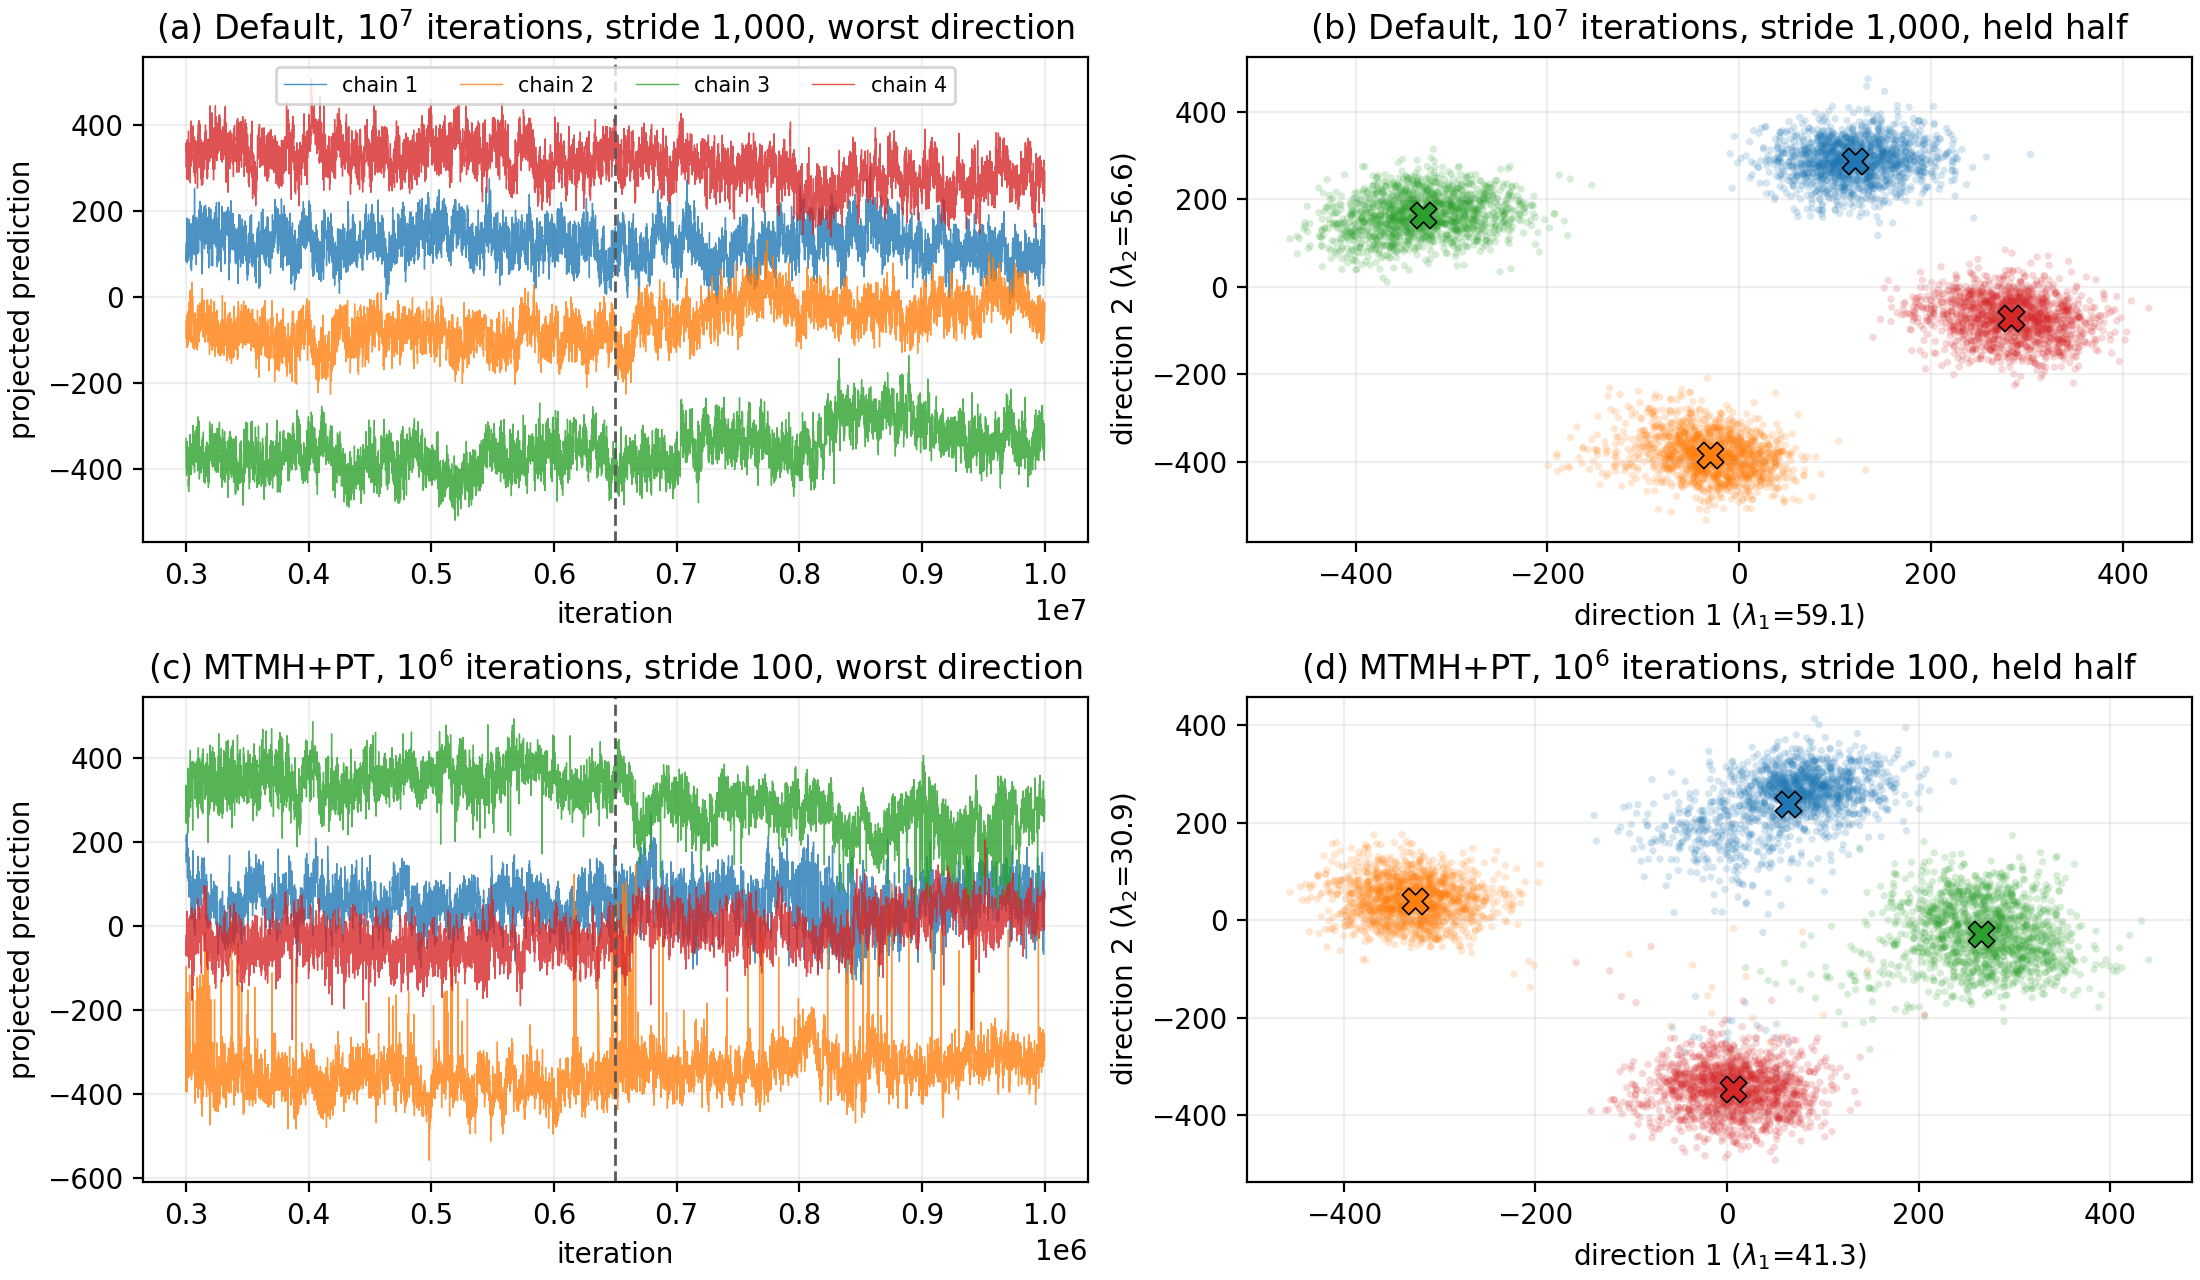
\includegraphics[width=\linewidth]{long_pt_worst2.png}
\caption{SeoulBike run 0, thinned records after the first 30\% is discarded; upper row Default ($10^7$ iterations), lower row MTMH+PT ($10^6$ iterations). (a,c) Predictions of all four chains projected onto the leading generalized eigenvector $v_1$; the dashed line ends the first half, on which the directions are fitted. (b,d) Second-half draws projected onto $v_1$ and $v_2$; crosses mark the chain centroids. Each record has its own axes.\newline{\zhfont SeoulBike run 0，丢掉前 30\% 后的 thinned 记录；上行 Default（$10^7$ 次迭代），下行 MTMH+PT（$10^6$ 次迭代）。(a,c) 4 条链的预测投影到主广义特征向量 $v_1$ 上；虚线标出前一半的结束位置，方向是用前一半拟合的。(b,d) 后一半 draws 在 $v_1$、$v_2$ 上的投影，叉号是各链的中心。每组记录用各自的坐标轴。}}
\label{fig:long-worst}
\end{figure}

\textbf{Trajectories.} Figure~\ref{fig:long-trace} and Table~\ref{tab:long-traj} follow the whole run.
\begin{itemize}
\item The log posterior rises in every chain over the first half. Between the fifth and tenth $10^5$-iteration deciles, chain~1 stays within 10 nats, and chains 2--4 gain 59, 28 and 139 nats.
\item In the last decile, the four chain means span 118 nats.
\item $\sigma$ decreases from about 155 to 132--137, and the total number of splits grows from about 315 to 350--375.
\item The test RMSE of decile-mean predictions ranges from 240 to 306, with no common trend.
\item Mean adjacent exchange acceptance falls from 0.40 in the first chunk to 0.28--0.30 in the last. The ladder was searched for the 0.4 target on a 1,000-row pilot.
\end{itemize}

\begin{zhbox}
\textbf{轨迹。}图 \ref{fig:long-trace} 和表 \ref{tab:long-traj} 跟踪了整个运行过程。
\begin{itemize}
\item 前半程，所有链的对数后验都在上升。从第 5 个到第 10 个 $10^5$ 次迭代十分位，chain 1 的变化在 10 nat 以内，chain 2--4 又涨了 59、28 和 139 nat。
\item 最后一个十分位里，4 条链的均值相差 118 nat。
\item $\sigma$ 从约 155 降到 132--137，总分裂数从约 315 涨到 350--375。
\item 各十分位平均预测的测试 RMSE 在 240 到 306 之间，没有共同的变化趋势。
\item 相邻温度的平均交换接受率从第一块的 0.40 降到最后一块的 0.28--0.30。温度梯子是在 1,000 行的 pilot 上按 0.4 的目标搜索的。
\end{itemize}
\end{zhbox}


\begin{figure}[h]
\centering
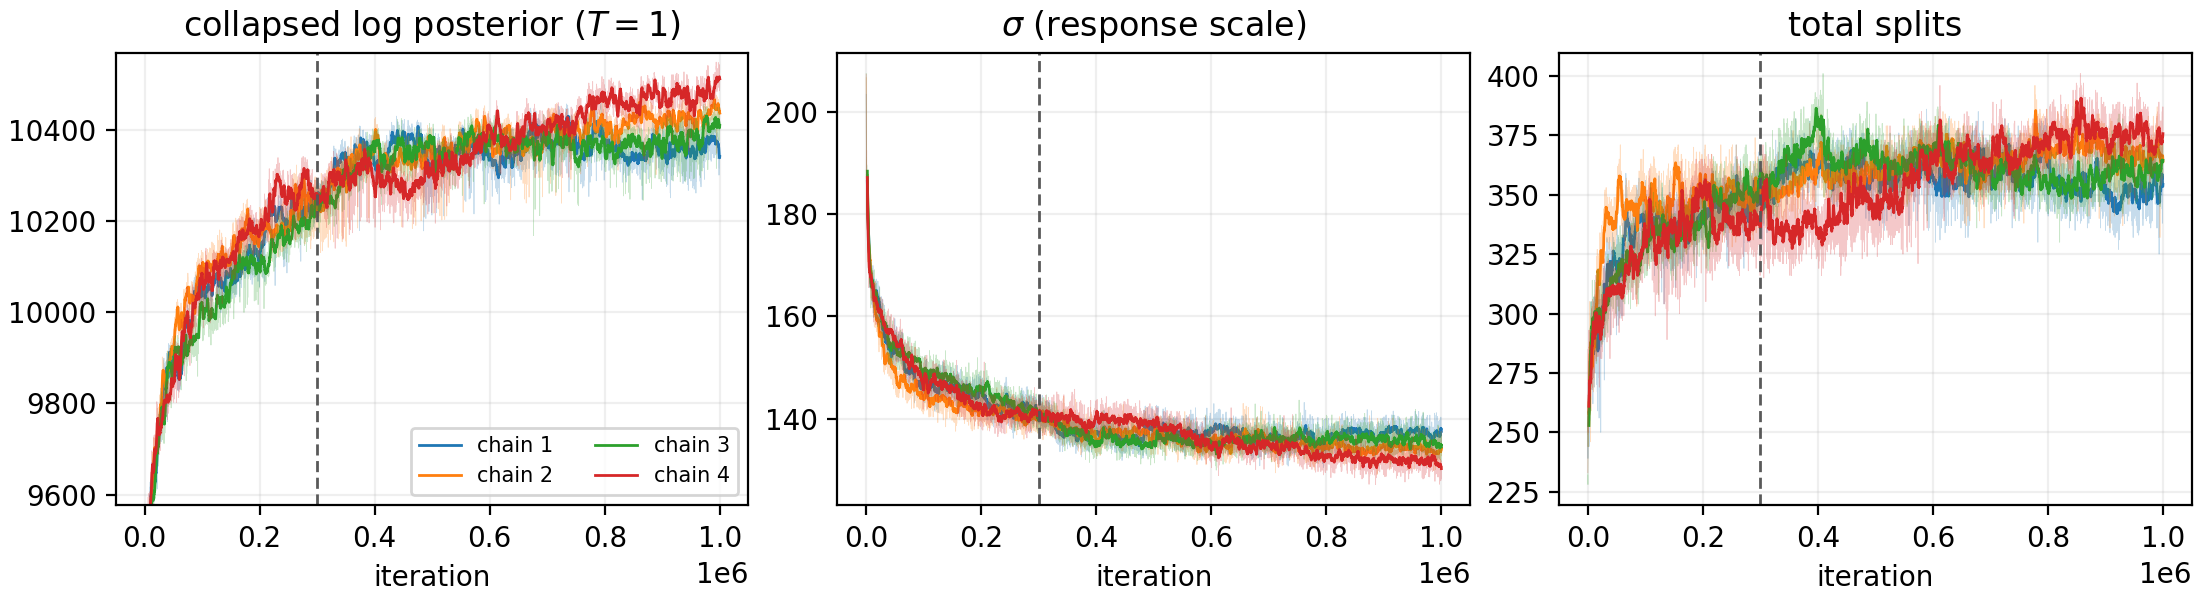
\includegraphics[width=\linewidth]{long_pt_traces.png}
\caption{Long MTMH+PT chains, SeoulBike run 0, every 100th iteration (faint) with a 20-draw moving average. The dashed line marks the end of the discarded first 30\%.\newline{\zhfont SeoulBike run 0 的长 MTMH+PT 链：每 100 次迭代一个点（浅色），加 20 个 draws 的移动平均。虚线标出丢掉的前 30\% 的结束位置。}}
\label{fig:long-trace}
\end{figure}

\begin{table}[h]
\centering
\small
\caption{Long MTMH+PT chains, SeoulBike run 0: decile means (D1, D5, D10 are iterations 1--100k, 400k--500k and 900k--1M). The log posterior is collapsed and evaluated at $T=1$; $\sigma$ and RMSE are on the response scale.\newline{\zhfont SeoulBike run 0 长 MTMH+PT 链的十分位均值（D1、D5、D10 分别是第 1--100k、400k--500k 和 900k--1M 次迭代）。对数后验是 $T=1$ 下的 collapsed 对数后验；$\sigma$ 和 RMSE 都在响应尺度上。}}
\label{tab:long-traj}
\begin{tabular}{lccccccccccc}
\toprule
 & \multicolumn{3}{c}{log posterior} & \multicolumn{3}{c}{$\sigma$} & \multicolumn{3}{c}{total splits} & \multicolumn{2}{c}{test RMSE} \\
\cmidrule(lr){2-4}\cmidrule(lr){5-7}\cmidrule(lr){8-10}\cmidrule(lr){11-12}
Chain & D1 & D5 & D10 & D1 & D5 & D10 & D1 & D5 & D10 & D1 & D10 \\
\midrule
1 & 9{,}834 & 10{,}358 & 10{,}360 & 155.6 & 136.7 & 137.3 & 317 & 361 & 350 & 273 & 248 \\
2 & 9{,}868 & 10{,}339 & 10{,}428 & 152.5 & 137.2 & 134.2 & 332 & 359 & 366 & 266 & 276 \\
3 & 9{,}807 & 10{,}353 & 10{,}389 & 156.8 & 135.6 & 135.6 & 311 & 367 & 360 & 250 & 291 \\
4 & 9{,}831 & 10{,}285 & 10{,}478 & 156.6 & 139.7 & 131.8 & 309 & 344 & 375 & 254 & 297 \\
\bottomrule
\end{tabular}
\end{table}

\textbf{Summary.} After $10^6$ iterations the four chains are not stationary: the log posterior is still rising in three of them, and $\sigma$ is still falling in two. Their pointwise agreement is better than that of the $10^7$-iteration Default chains, but not better than that of the production PT chains, and remains far from 1. They cannot serve as a reference posterior for SeoulBike. This agrees with the position of SeoulBike in Table~\ref{tab:paper}, where it has the third-largest $\kappa$ among the paper settings.

\begin{zhbox}
\textbf{小结。}跑完 $10^6$ 次迭代后，4 条链还没有平稳：3 条链的对数后验仍在上升，2 条链的 $\sigma$ 仍在下降。它们的 pointwise 一致性比 $10^7$ 次迭代的 Default 链好，但不比生产长度的 PT 链好，而且离 1 还很远。所以它们不能作为 SeoulBike 的参考后验。这与 SeoulBike 在表 \ref{tab:paper} 中的位置一致：它的 $\kappa$ 在论文 setting 中排第三大。
\end{zhbox}


\section{Conclusions\quad{\zhfont 结论}}
\begin{enumerate}
\item Collapsing the leaves makes the log-likelihood cost of a structural change proportional to $\kappa=n/(1-R^2)$ per unit of unexplained variance. The tree prior, the proposal ratio and the leaf term do not grow with $\kappa$.
\item Across 48 settings, $\kappa$ orders Default mixing difficulty ($\rho=0.89$). The regression coefficients of $n$ and of the noise fraction agree within their standard errors when $1-R^2_{\mathrm{CV}}$ is used. Responses with equal $\kappa$ give equal $\Rhat$ whether observed or semi-synthetic.
\item $\kappa$ can be computed from a cross-validated fit before running MCMC. The same ordering appears in the $10^7$-iteration chains, and $\kappa$ predicts the settings that remain unresolved.
\end{enumerate}

\begin{zhbox}
\begin{enumerate}
\item 把叶子积分掉以后，一次结构改动的对数似然代价，按每单位未解释方差计，正比于 $\kappa=n/(1-R^2)$。树先验、提议分布之比和叶子项都不随 $\kappa$ 增长。
\item 在 48 个 setting 上，$\kappa$ 能排出 Default 的混合难度（$\rho=0.89$）。用 $1-R^2_{\mathrm{CV}}$ 时，$n$ 和噪声比例的回归系数在标准误范围内相等。$\kappa$ 相同时，观测响应和半合成响应给出相同的 $\Rhat$。
\item $\kappa$ 可以在跑 MCMC 之前，用一次交叉验证拟合算出来。$10^7$ 次迭代的链呈现同样的排序，$\kappa$ 也能预测哪些 setting 始终不收敛。
\end{enumerate}
\end{zhbox}


\textbf{Limitations.}
\begin{itemize}
\item The derivation is a scale argument. It assumes comparable barrier depths $\delta^\ast$ across datasets and does not give mixing times.
\item $\Rhat$ is measured at $10^4$ iterations for 48 settings and at $10^7$ for twelve.
\item The controlled settings use three runs, and acceptance rates use one chain per setting.
\item The relation is a monotone ordering with scatter, not a calibrated prediction. Near $\kappa\approx1.6\times10^4$, for example, $\Rhat$ ranges from 1.06 (CCPP sweep, $n=1{,}000$) to 1.30 (Airfoil).
\item The cross-validated noise fraction depends on the gradient-boosting fit. It overstates the noise fraction when many predictors are irrelevant, as in the DART settings.
\end{itemize}

\begin{zhbox}
\textbf{局限。}
\begin{itemize}
\item 推导只是尺度论证。它假设不同数据集的势垒深度 $\delta^\ast$ 相近，不给出混合时间。
\item $10^4$ 次迭代的 $\Rhat$ 覆盖 48 个 setting，$10^7$ 次迭代的只有 12 个。
\item 控制实验只有 3 个 run，接受率每个 setting 只用了一条链。
\item 这是带散点的单调排序，不是校准过的预测。例如在 $\kappa\approx1.6\times10^4$ 附近，$\Rhat$ 从 1.06（CCPP 扫描，$n=1{,}000$）到 1.30（Airfoil）不等。
\item 交叉验证的噪声比例依赖于梯度提升的拟合。当很多变量无关时（如 DART setting），它会高估噪声比例。
\end{itemize}
\end{zhbox}


\textbf{Files.} Scripts and summaries are in \texttt{diagnosis/kappa\_note/} (branch \texttt{kappa-note}). Long-chain output is in \texttt{/scratch/e1377027/long\_pt/fixed100\_SeoulBike/} on Vanda; the runner is \texttt{hpc\_opt/long\_pt.py}.

\begin{zhbox}
\textbf{文件。}脚本和汇总结果在 \texttt{diagnosis/kappa\_note/} (branch \texttt{kappa-note})。长链输出在 Vanda 的 \texttt{/scratch/e1377027/long\_pt/fixed100\_SeoulBike/}，运行脚本是 \texttt{hpc\_opt/long\_pt.py}。
\end{zhbox}

\begin{thebibliography}{9}
\bibitem[Tan et al.(2024)]{tan2024computational}
Y.~S. Tan, O.~Ronen, T.~Saarinen and B.~Yu.
\newblock On the computational efficiency of Bayesian additive regression trees: an asymptotic analysis.
\newblock arXiv:2406.19958, 2024.
\end{thebibliography}

\end{document}
